% Task 8: logins with a hash chain.
\documentclass[12pt,tikz,border=6pt]{standalone}
% Shared preamble of the task figures of Lecture 6. The colours are the slide roles of Lectures 6 to 8:
%   Alice sIndigo, Eve and Mallory sPink, the message / data sViolet, a secret value sAmber,
%   Bob / the server sTeal, the digest sBrown; mechanisms neutral dark; the unknown: orange dashed.
\usepackage{lmodern}
\usepackage[T1]{fontenc}
\renewcommand{\familydefault}{\sfdefault}
\usepackage{amsmath,amssymb}
\usepackage{xcolor}
\usepackage{fontawesome5}
\usetikzlibrary{arrows.meta, calc, positioning, fit, decorations.pathreplacing, backgrounds}

\definecolor{DeepBlue}{HTML}{283593}
\definecolor{AccentOrange}{HTML}{EB5A14}
\definecolor{nInk}{HTML}{37474F}
\definecolor{nLine}{HTML}{90A4AE}
\definecolor{nLight}{HTML}{CFD8DC}
\definecolor{nFill}{HTML}{ECEFF1}
\definecolor{aExec}{HTML}{43A047}
\definecolor{aWrite}{HTML}{E53935}
\definecolor{sIndigo}{HTML}{5C6BC0}
\definecolor{sPink}{HTML}{EC407A}
\definecolor{sViolet}{HTML}{7E57C2}
\definecolor{sAmber}{HTML}{FFB300}
\definecolor{sTeal}{HTML}{26A69A}
\definecolor{sBrown}{HTML}{8D6E63}
\definecolor{sPinkText}{HTML}{C2185B}
\definecolor{sAmberText}{HTML}{A06A00}
\definecolor{sTealText}{HTML}{00796B}

\tikzset{
  hw/.style={draw=nLine, thick, fill=nFill, text=nInk, rounded corners=3pt, align=center, inner sep=4pt},
  hwmain/.style={draw=nInk, thick, fill=nInk, text=white, rounded corners=3pt, align=center, inner sep=5pt, font=\small\bfseries},
  msgval/.style={draw=sViolet, thick, fill=sViolet!12, text=nInk, rounded corners=3pt, align=center, inner sep=5pt},
  dgval/.style={draw=sBrown, thick, fill=sBrown!15, text=nInk, rounded corners=3pt, align=center, inner sep=5pt},
  secval/.style={draw=sAmber, thick, fill=sAmber!25, text=nInk, rounded corners=3pt, align=center, inner sep=5pt},
  unk/.style={draw=AccentOrange, thick, dashed, fill=white, text=AccentOrange, rounded corners=3pt, align=center,
    inner sep=5pt, font=\bfseries},
  data/.style={-{Stealth}, very thick, nInk},
  person/.style={circle, fill=#1, draw=#1, text=white, minimum size=1.1cm, font=\Large, inner sep=0pt},
}
\newcommand{\personnode}[4]{%
  \node[person=#3] (#1) at (#2) {\faUser};
  \node[font=\small\bfseries, text=#3, below=0.06cm of #1] (#1lbl) {#4};}
\newcommand{\mallorynode}[2]{%
  \node[person=sPink] (#1) at (#2) {\faUserNinja};
  \node[font=\small\bfseries, text=sPinkText, below=0.06cm of #1] (#1lbl) {Mallory};}
\newcommand{\evenode}[2]{%
  \node[person=sPink] (#1) at (#2) {\faUserSecret};
  \node[font=\small\bfseries, text=sPinkText, below=0.06cm of #1] (#1lbl) {Eve};}
\newcommand{\hashnode}[3]{\node[hwmain, minimum width=2.2cm, minimum height=0.9cm] (#1) at (#2) {\faCogs\ #3};}

\begin{document}
\pagecolor{white}
\begin{tikzpicture}[>=Stealth]
  \personnode{alice}{-1.4,0}{sIndigo}{Alice}
  \node[secval, font=\small] (x0) at (0.4,0) {$x_0$};
  \foreach \k/\x in {1/2.0, 2/3.6} \node[dgval, font=\small] (x\k) at (\x,0) {$x_\k$};
  \node[font=\large] (dots) at (5.0,0) {$\cdots$};
  \node[dgval, font=\small] (x99) at (6.4,0) {$x_{99}$};
  \node[dgval, font=\small] (x100) at (8.1,0) {$x_{100}$};
  \draw[data] (x0) -- node[above, font=\scriptsize] {H} (x1); \draw[data] (x1) -- node[above, font=\scriptsize] {H} (x2);
  \draw[data] (x2) -- (dots); \draw[data] (dots) -- (x99); \draw[data] (x99) -- node[above, font=\scriptsize] {H} (x100);
  \node[font=\scriptsize, text=gray, anchor=north] at (x0.south) {secret seed};
  \node[draw=sTeal, thick, fill=sTeal!15, text=nInk, rounded corners=3pt, align=center, inner sep=5pt, font=\small, minimum width=3.0cm] (srv) at (11.2,0) {\faServer\ Bob's server\\ \scriptsize stores $x_{100}$};
  \draw[data, dashed, nLine] (x100) -- (srv);
  \foreach \k in {1,...,5} \node[unk, font=\scriptsize, anchor=west] at (9.8,{-0.9-0.6*\k}) {login \k: OK or REJECTED?};
  \mallorynode{mal}{6.6,-2.6}
  \node[font=\scriptsize, text=sPinkText, anchor=west, align=left] at (7.3,-2.6) {listens and\\ sends logins too};
\end{tikzpicture}
\end{document}
